%!TEX ROOT=sample-thesis.tex
%!TEX PROGRAM=xelatex

% Sample thesis using FCIthesis.cls
% Developed by Jackel Chew (jackelchew93@ums.edu.my)

\documentclass[microtype]{FCIthesis}
    
% Load any other packages you need here
\usepackage{array}
\usepackage{booktabs}
\usepackage{graphicx}
\usepackage{siunitx}
\usepackage{xcolor}
\usepackage{nameref}

% Information about your thesis
\title{VISUAL ANALYTIC DESIGN FOR MASSIVELY OPEN ONLINE COURSES (MOOCS)}
\author{MOHAMMAD FADHLI BIN ASLI}
\matric{DI1711003T}
\degree{DOCTOR OF PHILOSOPHY}
\studyfield{INFORMATION TECHNOLOGY}
\faculty{FACULTY OF COMPUTING AND INFORMATICS}
\submissionyear{2021}
\vivadate{23 March 2021}

\begin{document}
\frontmatter

% Generates the cover page, a blank page, and then the title page
\makecoverandtitlepage

% Candidate's Declaration (remember to sign!)
\makedeclaration{5 July 2021}

% Supervisor's Declaration (remember to sign!)
\begin{SVdeclaration}
\member{Main Supervisor}{Dr. Muzaffar Hamzah}
\member{Co-Supervisor}{Assoc. Prof. Dr. Ag Asri Ag Ibrahim}
\end{SVdeclaration}

% Acknowledgement
%!TEX ROOT=sample-thesis.tex
%!TEX PROGRAM=xelatex

\begin{acknowledgement}[5 July 2021]
All praise is due to Allah, the Most Gracious and Most Merciful for the completion of this thesis. This entire journey would not be possible if it were not by His Grace. I hope that every knowledge and experience granted from this journey helps me to become a better human.
\\ \\ \noindent
To my beloved mother and father, once again, I owe everything to you from the very beginning. To my younger brother, thank you for being present when things get challenging. I truly appreciate all your love, patience, and support throughout this journey. I hope this achievement will make you guys proud.
\\ \\ \noindent
I would like to express the utmost gratitude to my supervisors, Dr. Muzaffar Hamzah and Assoc. Prof. Dr. Ag Asri Ag Ibrahim. Thank you so much for your endless effort and guidance throughout this research. I really appreciate every wisdom, knowledge, and trust that you have given to me, it helps me to become a better person.
\\ \\ \noindent
Lastly, I also would like to thank everyone who has supported this research. To all participants, without your utmost and discreet cooperation, this research could not be completed. To faculty members, thank you for sharing every insight, experience, and information that is beneficial for this research and my postgraduate learning.

\end{acknowledgement}

% English and Malay abstracts
\inputEnAbstract{sample-abstract}
\inputMsAbstract{sample-abstrak}

% List of Contents
{
	\clearpage
	\setstretch{1.5}
	\tableofcontents\clearpage	% Table of Contents
	\listoftables\clearpage		% List of Tables
	\listoffigures\clearpage		% List of Figures
%	\input{abbrevlist}\clearpage % List of Abbreviations
%	\input{symbollist}\clearpage	% List of Symbols
	\listofappendices\clearpage	% List of Appendices
}

\mainmatter
% All Chapters
%!TEX ROOT=sample-thesis.tex
%!TEX PROGRAM=xelatex

\chapter{Introduction}

This chapter introduces readers to the main purpose of conducting this study. First, motivations and significant events for undertaking this study are explained. Next, the statement of problem and objectives of this study are presented. Furthermore, proposed methodology to achieve the objectives and the research scope are described and characterized. Finally, a description on the layout of this thesis is presented.
\\[\baselineskip]\indent
The remainder of this chapter is as follows. Section 1.1 explain the motivations for carrying out this study. Description of the statement of problem for this study is presented in Section 1.2. Section 1.3 then describe the statement of objectives. In Section 1.4, detailed descriptions of methods to achieve the research objectives is presented followed by scopes and limitations in Section 1.5. Finally, this chapter present the layout of this thesis in Section 1.6.

\section{Motivations}
Three motives that encourage the study undertaken in this thesis are explained as follows.
\begin{itemize}
	\item \textbf{Rise of digitalization and big data calls for digital-capable society.} \\
Rapid escalation of digitalization and big data were observed over the years that signal the society’s transition into information era. These events call for efforts in supporting digital citizen development in many areas such as healthcare, communication, and education. This thesis refers digital citizen as an individual capable in utilizing information technology in real-world scenario. It was speculated that the deferral in digital citizen development can potentially diminishes society advances \parencite{Carrasco2017}. In order to support this development, improving method for enabling user to gain information and insight from data is considered to be necessary.  
	\item \textbf{National transition towards Education 4.0 by empowering educational technology adaptation.} \\
Malaysia is now embracing digital technology as part of the fourth Industrial Revolution (IR4.0), intensifying efforts on Education 4.0 advances. Education 4.0 is defined as the use of technology in teaching and learning context \parencite{Dunwill2016}. Transforming education is one of IR4.0 challenges and the Malaysia Education Blueprint for Higher Education was proposed to address this challenge. The national blueprint emphasizes on advancing online learning platform and resources such as e-Learning and MOOC. Massive open online course (MOOC) is introduced and implemented in Malaysia on 2013 \parencite{Ally2019}. Literature characterize Malaysian MOOC as exploratory and most related work were specifically focused on MOOC’s acceptance, perception, and effectiveness \parencite{Ayub2018}. This event highlights the need to empower the readiness for MOOC education transition in Malaysia. Further inaction likely increases the gap in educational technology adaptation between Malaysia and global education.
	\item \textbf{Limitation of pre-set analytics design hinders instructors in information and insight discovery.} \\
MOOC’s community is typically comprised of instructors, teaching assistants, and students. Community’s activities in MOOC enrolments and engagement generate large volume of data. These data contain potential insights for instructors in discovering pattern and behavior within their MOOC. Instructors gather these insights in order to improve their course’s contents. MOOC platforms such as Coursera, EdX, and OpenLearning can facilitate instructors with analytics to help their data exploration. However, the pre-set analytics have limitation in presenting information specifically involving large volume of data.
\end{itemize}

\section{Statement of Problem}
... 
\\[\baselineskip]\indent


\section{Statement of Objectives}
...
\\[\baselineskip]\indent

\section{Proposed Methodology}
To achieve the aim and objectives, this study used the following methodology and process as illustrated in Figure \ref{framework}. Each step of research activity is discussed as follows.

\begin{figure}[hbt!]
\centering
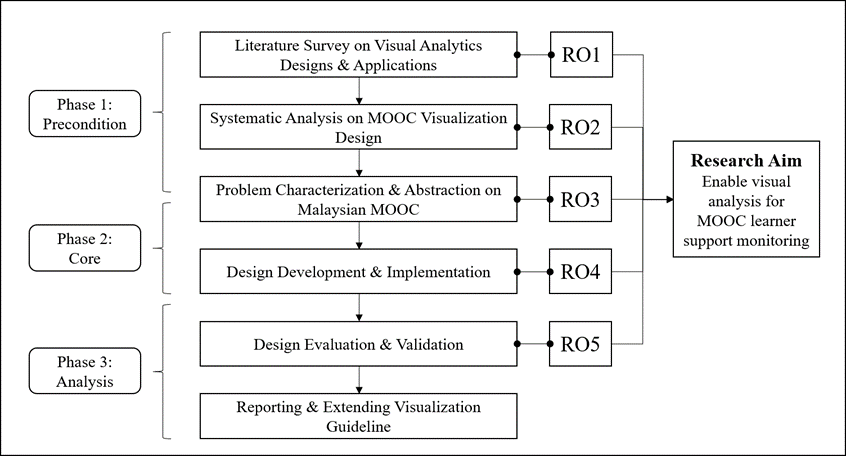
\includegraphics[scale=1]{Fig1.1}
\caption{Research framework of this study}
\label{framework} % to give the figure you want to reference a marker
\end{figure}

\medskip

\begin{enumerate}
\item A comprehensive literature survey and analysis of the recent visual analytics advances are undertaken to identify the current state of visual analytics designs and applications referring to scholarly digital libraries, particularly Scopus, IEEE Xplore, and ACM DL. This study also examines and classifies recent advances based on applied domains, design features, information-seeking tasks, data properties, data sources, and visualization techniques. The most significant design problems are identified to be addressed in this study.
\item The highlighted design problems are further investigated and verified its significance by further exploring the visualization design space of visual analytics designs and applications for MOOC data. A systematic analysis on existing MOOC visualization design is carried out by examining the reported analytic tasks, design requirements, data dimensions, visualization, and evaluation method. The resulting review helps elicit the visualization design  
\end{enumerate}

\begin{figure}[hbt!]
\centering
\begin{minipage}{0.3\textwidth}
\centering

\includegraphics[width=\linewidth]{green}
\subcaption{First subfigure}
\end{minipage}
%
\hspace{1cm}
%
\begin{minipage}{0.3\textwidth}
\centering
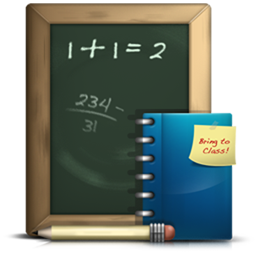
\includegraphics[width=\linewidth]{school}
\subcaption{Second subfigure}
\end{minipage}
\caption{An example with several subfigures}
\end{figure}

%!TEX ROOT=sample-thesis.tex
%!TEX PROGRAM=xelatex

\chapter{Literature Review}

This chapter reviews visualization literature to outline the state of the art, taxonomy, and emerging trends of visual analytics designs and applications. A thematic taxonomy of visual analytic designs and applications was devised to guide deriving the state of the art. The taxonomy classifies visual analytics studies according to applied domains, design features, information-seeking tasks, data properties, data sources, and visualization techniques. Furthermore, summarization of the design challenges and solutions for visual analytics were highlighted. Several design challenges in reported visual analytics including visual usability and information appertains are identified. In addition, a summarization of visual analytics for MOOC and case scenarios for this study is presented. Subsequently, this chapter explores the visualization design space of visual analytics designs and applications for MOOC data. A visualization design space of visual analytics for MOOC data is elicited based on the systematic review. The design space is then explored to identify and highlight the gaps or pitfalls in the current design guideline.
\\[\baselineskip]\indent
The remainder of this chapter is as follows. Section 2.1 introduces the underlying principles and definitions in the field of visualization. Section 2.2 then discusses the state of the art of visual analytics designs and applications. In Section 2.3, a taxonomy of visual analytics designs and applications and their characterization are introduced. Section 2.4 then highlights identified design challenges, while recommendations for these challenges are presented in Section 2.5. In Section 2.6, the relations between design challenges with the case of visual analytics for MOOC data are articulated. Section 2.7 then introduces the underlying principles of visualization design space, followed by Section 2.8 that presents a systematic analysis of MOOC visualization design. Finally, the chapter is concluded in Section 2.9.


\section{Foundation and Theories of Visualization and Visual Analytics}
This section presents the comprehensive analysis results of potential research gaps highlighted from the literature review. Furthermore, potential research gaps based on the relation with the motivation of this study are discussed. Moreover, a prime research gap is selected and discussed as the central motivation of this study. Subsequently, the justifications on the importance of dealing with the selected research gap were presented.

\subsection{Information Visualization and Visual Analytics}
Visualization is the representation of an object, situation, or set of information in the form of visual such as chart or graph \parencite{Oxford2020}. Visualization is also defined as the formation of human cognitive mental visual images, or the activity of interpreting in visual terms or of realizing it into visible form \parencite{Merriam2020,Owen1999}. This definition is then extended as “a tool or method for interpreting image data fed into a computer and for generating images from complex multi-dimensional data sets” \parencite{Owen1999}. Visualization techniques have been traditionally categorized into two major areas:
\begin{itemize}
\item Scientific visualization – visualization that involves scientific data with an inherent physical component.
\item Information visualization – visualization that involves abstract, nonspatial data.
\end{itemize}

\indent Information visualization is also known as the study of visual representations of abstract information to amplify the human cognition. When human is engaged through interaction with visual object (what they see with their eyes), there is an internal mental construction of information processing in their mind. Generally, visualization is a cognitive activity that is facilitated by external visual representations where human build an internal mental representation of it. Visual representations such as pictorials, graphs, and symbols help us to understand the external data thus producing better information understanding \parencite{Mazza2009}. The visualization process starts with refining or filtering the raw data, which then classified into data tables. The data then undergo visual structuring and then presented in the appropriate views \parencite{Card1999}. The whole process was shown in the Figure \ref{visual}. \\

\begin{figure}[hbt!]
\centering
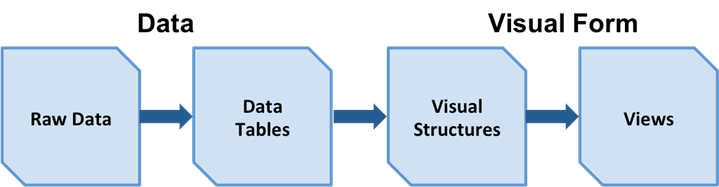
\includegraphics[scale=1]{Fig2.1}
\caption[Information visualization model]{Information visualization model\\\source{Card (1999)}}
\label{visual}
\end{figure}

\indent Visual analytics is a science of analytical reasoning facilitated by interactive visual interfaces. This thesis assert “interaction” as the key role of visual analytics as it facilitates interactivity between automated data analysis, visualization, and human user. Visual analytics enables human user to gain insights into solving complex problems by leveraging domain knowledge and intuition input with computer processing prowess. The exponential growth in data analytics utilization and visually driven data across many domains contributes to the rising need for effective visual analytics.

%!TEX ROOT=sample-thesis.tex
%!TEX PROGRAM=xelatex

\chapter{Methodology}

This chapter presents the detailed descriptions and justifications of the methodology used to achieve the research objectives. This chapter explains the methods used in this study into three major sections: problem characterization and abstraction, design development and implementation, and design evaluation and validation. Detailed characterization and abstraction of domain problems helps in deriving design requirements in generating appropriate visualization solutions. A literature review and a case study were carried out to elicit a problem abstraction based on data, users, and tasks. A visual analytics design was designed based on the identified requirements from the characterization and abstraction. Design experience on constructing the design including design consideration and rationales are also discussed. Finally, this chapter then introduces the user study methodology to evaluate and validate the design. Detailed descriptions of the user study methodology including think-aloud observation and expert validation interview are elaborated.
\\[\baselineskip]\indent
This chapter is organized as follows. Section 3.1 presents the domain problem characterization and abstraction for MOOC analytics. Detailed descriptions including the fundamentals of problem characterizations, user study methodology, and characterizations results are presented. In Section 3.2, detailed characteristics of domain and user requirements including data descriptions, tasks, and target user are described. Subsequently, design experience on the proposed design including design consideration and rationales to facilitate each domain problem are discussed. Section 3.3 then introduces the user case study methods used for evaluating and validating the proposed design. Detailed descriptions and justifications of protocols and instruments for think-aloud observation and expert validation are presented. Lastly, the chapter is concluded in Section 3.4.

\section{Problem Characterization and Abstraction for MOOC Analytics}
This section firstly introduces the concept and example studies of problem characterization and abstraction. Next, discussions on related literature on visual analytics and visualization for MOOC are presented. Subsequently, detailed descriptions of case study method to extract domain problem characterization and abstraction are described. This section then presents and discuss the findings from the problem characterization to be design references in facilitating MOOC learner support monitoring.

\subsection{Problem Characterization and Abstraction}
There are limited existing visualization research focusing on problem-oriented visualization despite its importance in visual analytics design and implementation (Lam et al., 2012). To encourage problem-oriented approach in visualization, the design study methodology is introduced \parencite{Sedlmair2012}. This methodology leverages detailed problem characterization and abstraction in designing visual analytics solution. Notable examples of problem characterization and abstraction in design studies across domains are discussed as follows.
\\[\baselineskip]\indent
\textcite{Wagner2014} investigated the design requirements of visual analytics for behavior-based malware pattern analysis \parencite{Wagner2014}. They characterized the design requirements based on problem characterization and abstraction using literature, user focus groups, and expert interviews.
\\[\baselineskip]\indent
\textcite{Riveiro2017} then conducted a design study on facilitating visual analysis in anomaly detection on multidimensional transport traffic data \parencite{Riveiro2017}. Their design framework was implemented and demonstrated on European real transport traffic data. Furthermore, expert analysts from industrial organization were interviewed for evaluating the usability of the proposed design framework.

\begin{figure}[hbt!]
\centering
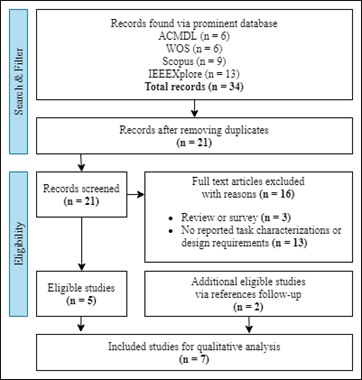
\includegraphics[scale=1]{Fig3.2}
\caption{Literature review workflow for problem characterizations}
\end{figure}

\bigskip

\begin{table}[hbt!]
\caption{Inclusion and exclusion criteria for literature selection for review}
\centering
\begin{tabular}{ p{1.5cm} p{5cm} p{6.5cm} }
\hline
No.	& Criteria & Justification \\ \hline
1 	& The study must be an original research paper instead of a review or survey paper. & Review and survey papers do not always contain a sufficient description of design studies or detailed problem characterizations. \\
\hline
\end{tabular}
\end{table}

\subsubsection{Expert Interview}
To help characterize domain analysis tasks and user requirements, several MOOC experts were recruited from the education field in Malaysia. An interview protocol was designed for the semi-structured interview sessions as follows.
\\ \\
a.	Identify \\
\indent $OI_1$ \indent Total number of learners in the course. \\
\indent $OI_2$ \indent Percentage of learners with age between 35 and 55 years old. \\
\indent $OI_3$ \indent Number of categories for learners’ academic background. \\
\indent $OI_4$ \indent List 3 learners who completed the course with distinction.
\\ \\
b.	Find extremum \\
\indent $OE_1$ \indent Month with highest number of registrations, and then withdrawals. \\
\indent $OE_2$ \indent Largest group of learners by their academic background. \\
\indent $OE_3$ \indent Smallest group of learners by their final grade.
\\ \\

\begin{table}[hbt!]
\caption{Justification of pre-defined tasks during analysis scenario on Overview view}
\centering
\begin{tabular}{ |c|c|c|c| }
\hline
Hey & How's it & Going?\\ \hline
Fine! & Just great. & See ya!\\
Fine! & Just great. & See ya!\\
\hline
\end{tabular}

\source{The Source.}
\end{table}

Time for some maths.
\begin{equation}
\left[M\frac{\partial }{\partial M}+\beta(g)\frac{\partial }{\partial g}+n\gamma\right] G^{(n)}(x_1,x_2,\ldots,x_n;M,g)=0,
\end{equation}

%!TEX ROOT=sample-thesis.tex
%!TEX PROGRAM=xelatex

\chapter{Results and Discussions}

In this chapter, the results of the user case study are presented and discussed to evaluate the proposed design. The recorded user activities in think-aloud observation were examined and discussed to identify user cognition sequence and behavior. The findings from the user case study then validated based on experts’ interview results. The perceptual usefulness and effectiveness of the proposed design including each view panels were further validated. Furthermore, discussions on the findings based on design fulfilment, domain user behavior, and design limitations are presented.
\\ \\ \indent
The remainder of this chapter is as follows. Section 4.1 present and discuss the results of think-aloud observation on each view. Section 4.2 discuss on expert validation towards findings from user case study. In Section 4.3, significant findings from the user case study are further discussed. Finally, the conclusion of this chapter is presented in Section 4.4.

\section{User Case Study Results}
This section presents and discusses the user case study results from the think-aloud observation with domain expert. Domain experts’ experience in performing MOOC analysis using the proposed visual analytics design are reported. This study then further examines their analysis activity on each view and thought process during the observation.

\subsection{User Cognition on Overview View}
Experts’ cognition experience when using the Overview features of the proposed visual analytics are examined and described in Table 4.1. The results of cognition experience on each task are discussed as follows.

\begin{table}[hbt!]
\caption{Cognition experience of domain experts in completing tasks using Overview}
\centering
\begin{tabular}{ ccccccc }
\hline
\textbf{Task} 	& \textbf{DE1} 	& \textbf{DE2} 	& \textbf{DE3} 	& \textbf{DE4} 	& \textbf{DE5} 	& \textbf{DE6} 	\\ \hline
\multicolumn{7}{l}{\textbf{Identify}}	\\ \hline
$OI_1$			& Moderate 		& Easy 			& Easy 			& Easy 			& Easy 			& Easy 			\\ 
$OI_2$			& Easy 			& Easy 			& Easy 			& Easy 			& Moderate 		& Easy 			\\ 
$OI_3$			& Moderate 		& Easy 			& Easy 			& Easy 			& Easy 			& Moderate 		\\ 
%\multicolumn{7}{|l|}{} \\
%\multicolumn{7}{|l|}{\textbf{Find Extremum}} \\ \hline
$OE_1$	& Easy & Easy & Easy & Moderate & Easy & Moderate 	\\ 
$OE_2$	& Easy & Easy & Easy & Easy & Easy & Easy 	\\ 
$OE_3$	& Moderate & Easy & Easy & Easy & Easy & Easy \\
%\multicolumn{7}{|l|}{} \\
%\multicolumn{7}{|l|}{\textbf{Compare}} \hline
$OC_1$			& Moderate 		& Easy 			& Moderate 		& Moderate 		& Easy 			& Moderate 		\\ 
$OC_2$			& Moderate 		& Easy 			& Easy 			& Moderate 		& Easy 			& Moderate 		\\ 
$OC_3$			& Moderate 		& Easy 			& Easy 			& Easy 			& Easy 			& Easy 			\\
\hline
\end{tabular}
\end{table}

\subsubsection{Identify}
\textbf{$OI_1$: Identify total number of learners in the course} \\
Generally, all participant was able to accomplish this task. However, few participants require additional time to recognize the presented information. In this task scenario, it was found that the use of color, size, and positioning is crucial in rendering first-hand information. Expert 1 remarked \textit{“I browsed until the bottom. I thought that perhaps it looks like accounting statement, with great total”}. However, this study considered it as uncommon scenario since the other participants were able to identify the item from top. Moreover, this study learns that appropriate use of colors without compromising cognition attention is crucial in presenting overview information. Expert 4 expressed excitement towards the colors in the panel, but she mistaken the values in colored legend as total learners. Furthermore, Expert 1 commented \textit{“Since the total number of learners is important, if it was red-colored, I will definitely be able to recognize it. Not gray though.”}. These findings on colors utilization correlates with previous work that emphasizes on effective color mapping.
\\[\baselineskip]\indent
Time for some maths.

\begin{equation}
\left[M\frac{\partial }{\partial M}+\beta(g)\frac{\partial }{\partial g}+n\gamma\right] G^{(n)}(x_1,x_2,\ldots,x_n;M,g)=0,
\end{equation}

%!TEX ROOT=sample-thesis.tex
%!TEX PROGRAM=xelatex

\chapter{Conclusions and Future Works}

This chapter presents the conclusions and the identified future works of this thesis. This chapter firstly describes how the aim and objectives of this study are fulfilled. Next, the contributions of this thesis and the significance of the work carried out in this study are highlighted. Lastly, this chapter describes the limitations of this study and suggests possible future works.
\\ \\ \indent
The remainder of this chapter is as follows. In Section 5.1, the accomplishment of the aim and objectives of this study are described. Section 5.2 then highlights the contributions of this thesis. Section 5.3 presents the significance of this work. Finally, the limitations and future works are discussed in Section 5.4.

\section{Aim and Objectives Achievement}
This study aimed to enable visual analysis for facilitating instructors in MOOC learner support monitoring using visual analytics. This section explains how the research aim was attained by accomplishing the following objectives.

\subsection{Investigate the recent visual analytics designs and applications to identify current design gap}
This study accomplished this objective by reviewing the most credible published visualization studies via scholarly databases. Recent visualization literature published in the most prominent visualization journals and conferences were visited and thoroughly examined. This study then analyzed and classified the recent visual analytics designs and applications and identify four design challenges: visual usability, scalability, interactivity, information appertains.



% References
\printbibliography[heading=customheading]

% Appendix
\appendix
%!TEX ROOT=sample-thesis.tex
%!TEX PROGRAM=xelatex

\chapter{Problem Characterization Interview Sample}

\begin{table}[hbt!]
\centering
\begin{tabular}{|p{3cm}|p{9.5cm}|} % max 12.5cm
	\hline
	Questions & Voice remarks (\textcolor{blue}{Researcher = Blue}, Experts = Dark) \\
  	\hline
  	\multicolumn{2}{|c|}{Problem Characterization} \\
  	\hline
	Q1 & Okay, mine is basically task-based, it was not content-based. all the modules are pretty much task-oriented, so there are tasks to be completed. if we look at the old version, it looks similar to the forum when the learner completed the tasks. the form is like there is a video, and there are discussions attached to it. because mine is self-paced, people respond to the tasks, it is not meant for them to discuss in the forum, it is meant for them to go to the tasks, it just that it is more task-based. however, if somebody wants to read other people's comments, they want to comment, it is there. at a few levels, there are peers commenting on their tasks, that is it. but the whole design is not a forum. the whole design is for each of them to complete a task, so the task sometimes requires them to answer in sentences. but many of my tasks were also in a form of visual. they need to create and submit a poster, a mind map. so, the interaction happens there is like peers upvoting or 'like' their work. \newline
	\textcolor{blue}{That one is one of the activities that we intend to identify such as 'like', 'upvote'.} \\
  \hline
\end{tabular}
\end{table}


\end{document}